% Options for packages loaded elsewhere
% Options for packages loaded elsewhere
\PassOptionsToPackage{unicode}{hyperref}
\PassOptionsToPackage{hyphens}{url}
\PassOptionsToPackage{dvipsnames,svgnames,x11names}{xcolor}
%
\documentclass[
  letterpaper,
  DIV=11,
  numbers=noendperiod]{scrartcl}
\usepackage{xcolor}
\usepackage{amsmath,amssymb}
\setcounter{secnumdepth}{-\maxdimen} % remove section numbering
\usepackage{iftex}
\ifPDFTeX
  \usepackage[T1]{fontenc}
  \usepackage[utf8]{inputenc}
  \usepackage{textcomp} % provide euro and other symbols
\else % if luatex or xetex
  \usepackage{unicode-math} % this also loads fontspec
  \defaultfontfeatures{Scale=MatchLowercase}
  \defaultfontfeatures[\rmfamily]{Ligatures=TeX,Scale=1}
\fi
\usepackage{lmodern}
\ifPDFTeX\else
  % xetex/luatex font selection
\fi
% Use upquote if available, for straight quotes in verbatim environments
\IfFileExists{upquote.sty}{\usepackage{upquote}}{}
\IfFileExists{microtype.sty}{% use microtype if available
  \usepackage[]{microtype}
  \UseMicrotypeSet[protrusion]{basicmath} % disable protrusion for tt fonts
}{}
\makeatletter
\@ifundefined{KOMAClassName}{% if non-KOMA class
  \IfFileExists{parskip.sty}{%
    \usepackage{parskip}
  }{% else
    \setlength{\parindent}{0pt}
    \setlength{\parskip}{6pt plus 2pt minus 1pt}}
}{% if KOMA class
  \KOMAoptions{parskip=half}}
\makeatother
% Make \paragraph and \subparagraph free-standing
\makeatletter
\ifx\paragraph\undefined\else
  \let\oldparagraph\paragraph
  \renewcommand{\paragraph}{
    \@ifstar
      \xxxParagraphStar
      \xxxParagraphNoStar
  }
  \newcommand{\xxxParagraphStar}[1]{\oldparagraph*{#1}\mbox{}}
  \newcommand{\xxxParagraphNoStar}[1]{\oldparagraph{#1}\mbox{}}
\fi
\ifx\subparagraph\undefined\else
  \let\oldsubparagraph\subparagraph
  \renewcommand{\subparagraph}{
    \@ifstar
      \xxxSubParagraphStar
      \xxxSubParagraphNoStar
  }
  \newcommand{\xxxSubParagraphStar}[1]{\oldsubparagraph*{#1}\mbox{}}
  \newcommand{\xxxSubParagraphNoStar}[1]{\oldsubparagraph{#1}\mbox{}}
\fi
\makeatother

\usepackage{color}
\usepackage{fancyvrb}
\newcommand{\VerbBar}{|}
\newcommand{\VERB}{\Verb[commandchars=\\\{\}]}
\DefineVerbatimEnvironment{Highlighting}{Verbatim}{commandchars=\\\{\}}
% Add ',fontsize=\small' for more characters per line
\usepackage{framed}
\definecolor{shadecolor}{RGB}{241,243,245}
\newenvironment{Shaded}{\begin{snugshade}}{\end{snugshade}}
\newcommand{\AlertTok}[1]{\textcolor[rgb]{0.68,0.00,0.00}{#1}}
\newcommand{\AnnotationTok}[1]{\textcolor[rgb]{0.37,0.37,0.37}{#1}}
\newcommand{\AttributeTok}[1]{\textcolor[rgb]{0.40,0.45,0.13}{#1}}
\newcommand{\BaseNTok}[1]{\textcolor[rgb]{0.68,0.00,0.00}{#1}}
\newcommand{\BuiltInTok}[1]{\textcolor[rgb]{0.00,0.23,0.31}{#1}}
\newcommand{\CharTok}[1]{\textcolor[rgb]{0.13,0.47,0.30}{#1}}
\newcommand{\CommentTok}[1]{\textcolor[rgb]{0.37,0.37,0.37}{#1}}
\newcommand{\CommentVarTok}[1]{\textcolor[rgb]{0.37,0.37,0.37}{\textit{#1}}}
\newcommand{\ConstantTok}[1]{\textcolor[rgb]{0.56,0.35,0.01}{#1}}
\newcommand{\ControlFlowTok}[1]{\textcolor[rgb]{0.00,0.23,0.31}{\textbf{#1}}}
\newcommand{\DataTypeTok}[1]{\textcolor[rgb]{0.68,0.00,0.00}{#1}}
\newcommand{\DecValTok}[1]{\textcolor[rgb]{0.68,0.00,0.00}{#1}}
\newcommand{\DocumentationTok}[1]{\textcolor[rgb]{0.37,0.37,0.37}{\textit{#1}}}
\newcommand{\ErrorTok}[1]{\textcolor[rgb]{0.68,0.00,0.00}{#1}}
\newcommand{\ExtensionTok}[1]{\textcolor[rgb]{0.00,0.23,0.31}{#1}}
\newcommand{\FloatTok}[1]{\textcolor[rgb]{0.68,0.00,0.00}{#1}}
\newcommand{\FunctionTok}[1]{\textcolor[rgb]{0.28,0.35,0.67}{#1}}
\newcommand{\ImportTok}[1]{\textcolor[rgb]{0.00,0.46,0.62}{#1}}
\newcommand{\InformationTok}[1]{\textcolor[rgb]{0.37,0.37,0.37}{#1}}
\newcommand{\KeywordTok}[1]{\textcolor[rgb]{0.00,0.23,0.31}{\textbf{#1}}}
\newcommand{\NormalTok}[1]{\textcolor[rgb]{0.00,0.23,0.31}{#1}}
\newcommand{\OperatorTok}[1]{\textcolor[rgb]{0.37,0.37,0.37}{#1}}
\newcommand{\OtherTok}[1]{\textcolor[rgb]{0.00,0.23,0.31}{#1}}
\newcommand{\PreprocessorTok}[1]{\textcolor[rgb]{0.68,0.00,0.00}{#1}}
\newcommand{\RegionMarkerTok}[1]{\textcolor[rgb]{0.00,0.23,0.31}{#1}}
\newcommand{\SpecialCharTok}[1]{\textcolor[rgb]{0.37,0.37,0.37}{#1}}
\newcommand{\SpecialStringTok}[1]{\textcolor[rgb]{0.13,0.47,0.30}{#1}}
\newcommand{\StringTok}[1]{\textcolor[rgb]{0.13,0.47,0.30}{#1}}
\newcommand{\VariableTok}[1]{\textcolor[rgb]{0.07,0.07,0.07}{#1}}
\newcommand{\VerbatimStringTok}[1]{\textcolor[rgb]{0.13,0.47,0.30}{#1}}
\newcommand{\WarningTok}[1]{\textcolor[rgb]{0.37,0.37,0.37}{\textit{#1}}}

\usepackage{longtable,booktabs,array}
\usepackage{calc} % for calculating minipage widths
% Correct order of tables after \paragraph or \subparagraph
\usepackage{etoolbox}
\makeatletter
\patchcmd\longtable{\par}{\if@noskipsec\mbox{}\fi\par}{}{}
\makeatother
% Allow footnotes in longtable head/foot
\IfFileExists{footnotehyper.sty}{\usepackage{footnotehyper}}{\usepackage{footnote}}
\makesavenoteenv{longtable}
\usepackage{graphicx}
\makeatletter
\newsavebox\pandoc@box
\newcommand*\pandocbounded[1]{% scales image to fit in text height/width
  \sbox\pandoc@box{#1}%
  \Gscale@div\@tempa{\textheight}{\dimexpr\ht\pandoc@box+\dp\pandoc@box\relax}%
  \Gscale@div\@tempb{\linewidth}{\wd\pandoc@box}%
  \ifdim\@tempb\p@<\@tempa\p@\let\@tempa\@tempb\fi% select the smaller of both
  \ifdim\@tempa\p@<\p@\scalebox{\@tempa}{\usebox\pandoc@box}%
  \else\usebox{\pandoc@box}%
  \fi%
}
% Set default figure placement to htbp
\def\fps@figure{htbp}
\makeatother





\setlength{\emergencystretch}{3em} % prevent overfull lines

\providecommand{\tightlist}{%
  \setlength{\itemsep}{0pt}\setlength{\parskip}{0pt}}



 


\KOMAoption{captions}{tableheading}
\makeatletter
\@ifpackageloaded{caption}{}{\usepackage{caption}}
\AtBeginDocument{%
\ifdefined\contentsname
  \renewcommand*\contentsname{Table of contents}
\else
  \newcommand\contentsname{Table of contents}
\fi
\ifdefined\listfigurename
  \renewcommand*\listfigurename{List of Figures}
\else
  \newcommand\listfigurename{List of Figures}
\fi
\ifdefined\listtablename
  \renewcommand*\listtablename{List of Tables}
\else
  \newcommand\listtablename{List of Tables}
\fi
\ifdefined\figurename
  \renewcommand*\figurename{Figure}
\else
  \newcommand\figurename{Figure}
\fi
\ifdefined\tablename
  \renewcommand*\tablename{Table}
\else
  \newcommand\tablename{Table}
\fi
}
\@ifpackageloaded{float}{}{\usepackage{float}}
\floatstyle{ruled}
\@ifundefined{c@chapter}{\newfloat{codelisting}{h}{lop}}{\newfloat{codelisting}{h}{lop}[chapter]}
\floatname{codelisting}{Listing}
\newcommand*\listoflistings{\listof{codelisting}{List of Listings}}
\makeatother
\makeatletter
\makeatother
\makeatletter
\@ifpackageloaded{caption}{}{\usepackage{caption}}
\@ifpackageloaded{subcaption}{}{\usepackage{subcaption}}
\makeatother
\usepackage{bookmark}
\IfFileExists{xurl.sty}{\usepackage{xurl}}{} % add URL line breaks if available
\urlstyle{same}
\hypersetup{
  pdftitle={Preparation for Lab 1 - Northe, Velez, Wörner},
  colorlinks=true,
  linkcolor={blue},
  filecolor={Maroon},
  citecolor={Blue},
  urlcolor={Blue},
  pdfcreator={LaTeX via pandoc}}


\title{Preparation for Lab 1 - Northe, Velez, Wörner}
\author{}
\date{}
\begin{document}
\maketitle


The source code and the binaries from the spectrum analyzer from this
report can be found in our Github
\href{https://github.com/NortheLo/Microwave_Eng_Lab/tree/main/Lab1_Network_Analysis}{repository}.

\begin{Shaded}
\begin{Highlighting}[]
\ImportTok{import}\NormalTok{ matplotlib.pyplot }\ImportTok{as}\NormalTok{ plt}
\ImportTok{import}\NormalTok{ numpy }\ImportTok{as}\NormalTok{ np}
\end{Highlighting}
\end{Shaded}

\subsection{Task 1}\label{task-1}

The connection sketches are presented as follows: \#\#\# Filter:

\begin{figure}[H]

{\centering \pandocbounded{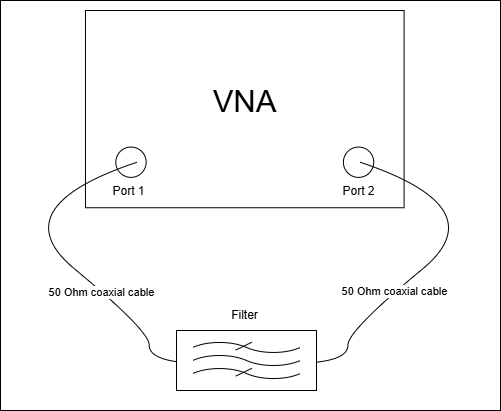
\includegraphics[keepaspectratio]{Prelim_Task1_Filter.png}}

}

\caption{Prelim\_Task1\_Filter.png}

\end{figure}%

\subsubsection{Circulator:}\label{circulator}

\begin{figure}[H]

{\centering \pandocbounded{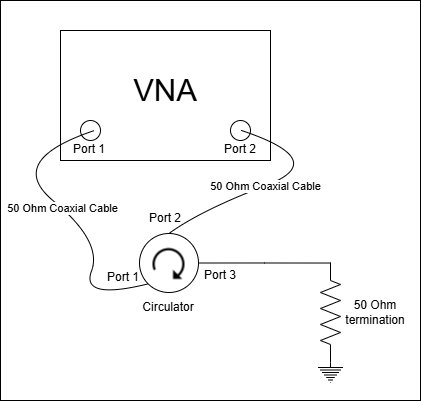
\includegraphics[keepaspectratio]{Prelim_Task1_Circulator.png}}

}

\caption{Prelim\_Task1\_Circulator.png}

\end{figure}%

\subsubsection{Coupler:}\label{coupler}

\begin{figure}[H]

{\centering \pandocbounded{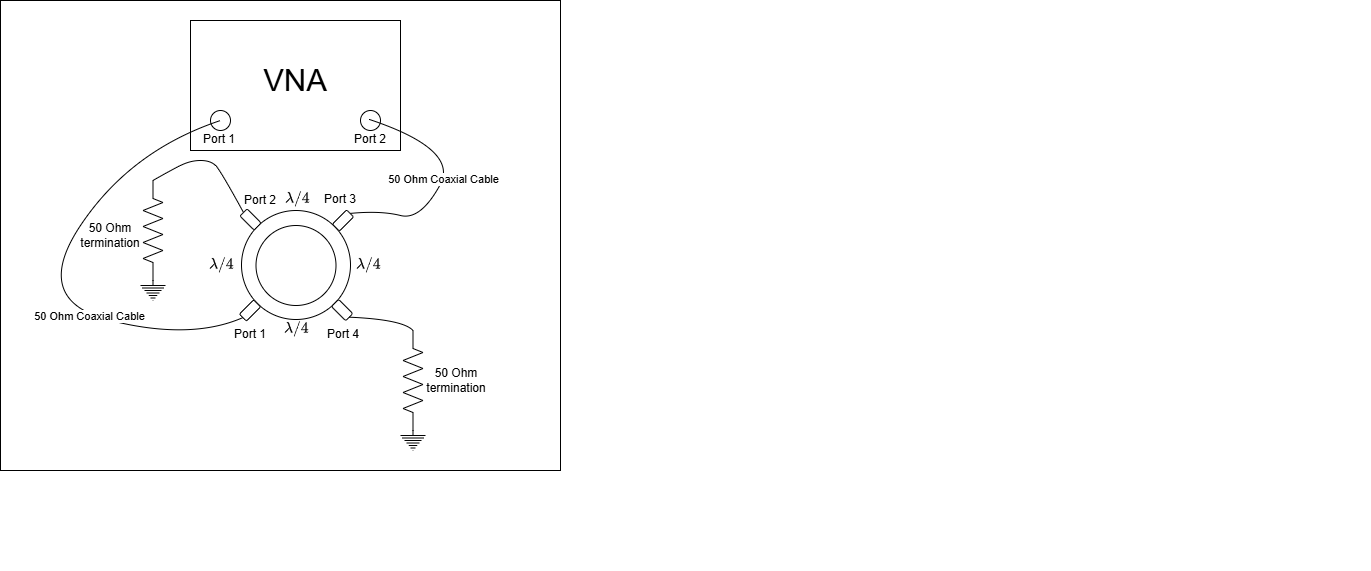
\includegraphics[keepaspectratio]{Prelim_Task1_Coupler.png}}

}

\caption{Prelim\_Task1\_Coupler.png}

\end{figure}%

\subsubsection{Line:}\label{line}

\begin{figure}[H]

{\centering \pandocbounded{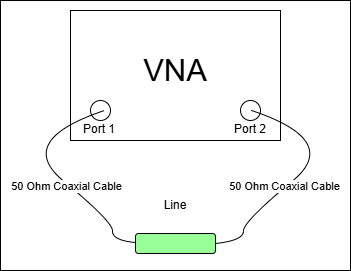
\includegraphics[keepaspectratio]{Prelim_Task1_Line.png}}

}

\caption{Prelim\_Task1\_Line.png}

\end{figure}%

\subsubsection{Wilkinson Divider:}\label{wilkinson-divider}

\begin{figure}[H]

{\centering \pandocbounded{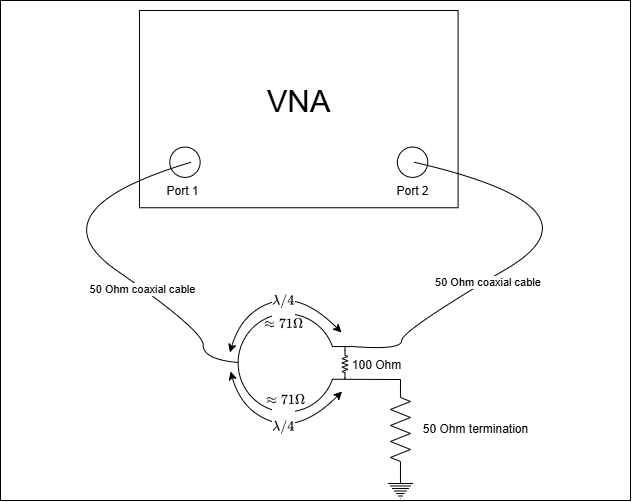
\includegraphics[keepaspectratio]{Prelim_Task1_Wilk_Div.png}}

}

\caption{Prelim\_Task1\_Wilk\_Div.png}

\end{figure}%

\subsection{Task 2}\label{task-2}

\subsubsection{a) Sketch the measurement setup of the amplifier
measurement, which is described in Task 8 of the experimental
tasks.}\label{a-sketch-the-measurement-setup-of-the-amplifier-measurement-which-is-described-in-task-8-of-the-experimental-tasks.}

\begin{figure}[H]

{\centering \pandocbounded{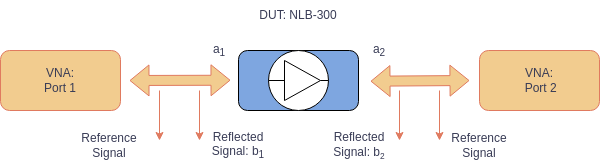
\includegraphics[keepaspectratio]{Prelim_Task3_Circuit.png}}

}

\caption{pic}

\end{figure}%

\subsubsection{b) Find maximum power levels according to specifications
of a network analyzer (input and
output).}\label{b-find-maximum-power-levels-according-to-specifications-of-a-network-analyzer-input-and-output.}

As there wasn't a specific model stated, we used this
\href{https://scdn.rohde-schwarz.com/ur/pws/dl_downloads/pdm/cl_brochures_and_datasheets/specifications/5215_4652_22/ZNA_specs_en_5215-4652-22_v2100.pdf}{Rohde
\& Schwarz ZNA67 datasheet}

\textbf{Output Test Port from page 24}

\begin{figure}[H]

{\centering \pandocbounded{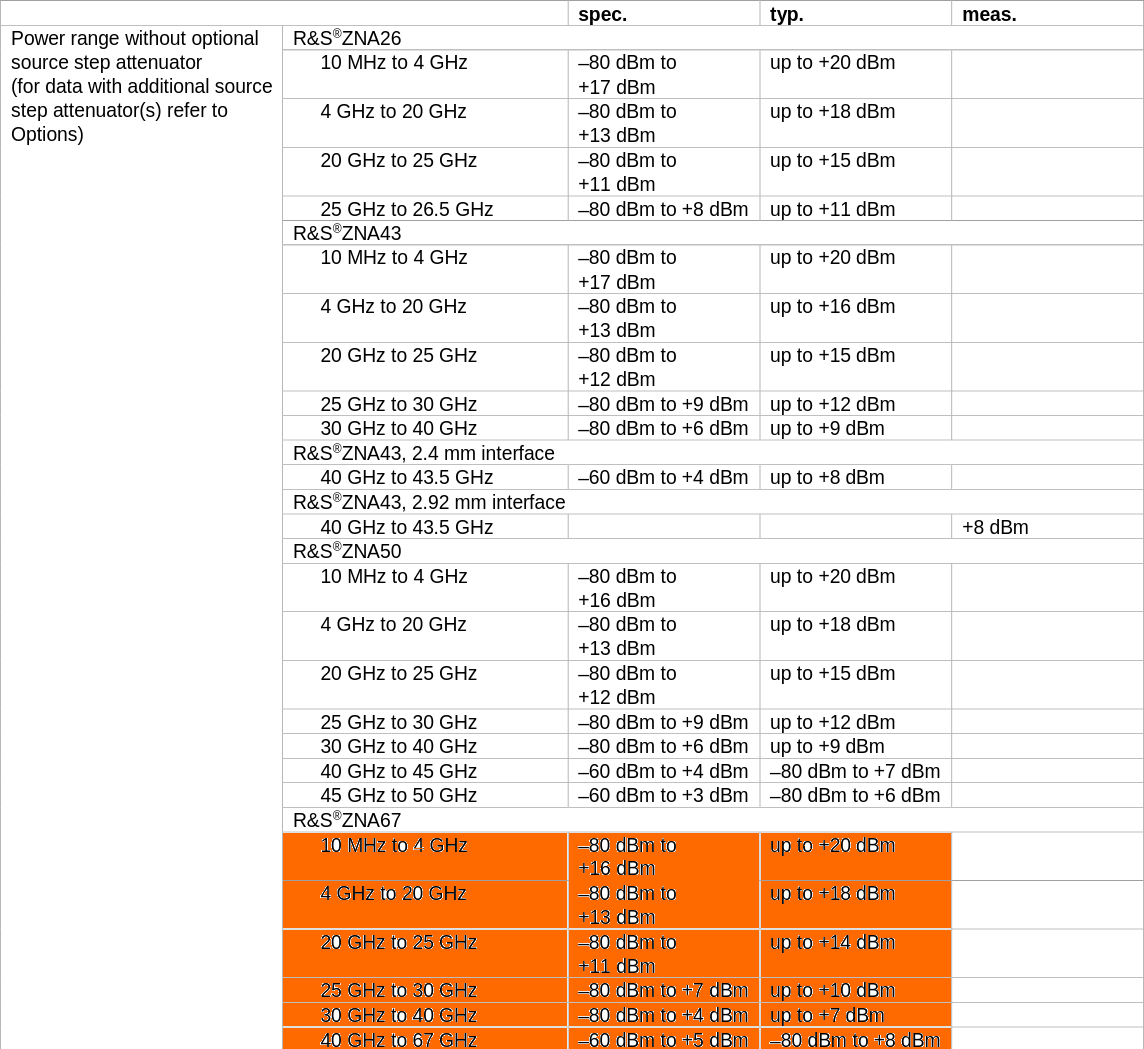
\includegraphics[keepaspectratio]{ZNA67_max_power_level.png}}

}

\caption{title}

\end{figure}%

\textbf{Maximum Input Level from page 27}

At \(+27dBm\) is the maximum power level, which can be accepted.

\begin{figure}[H]

{\centering \pandocbounded{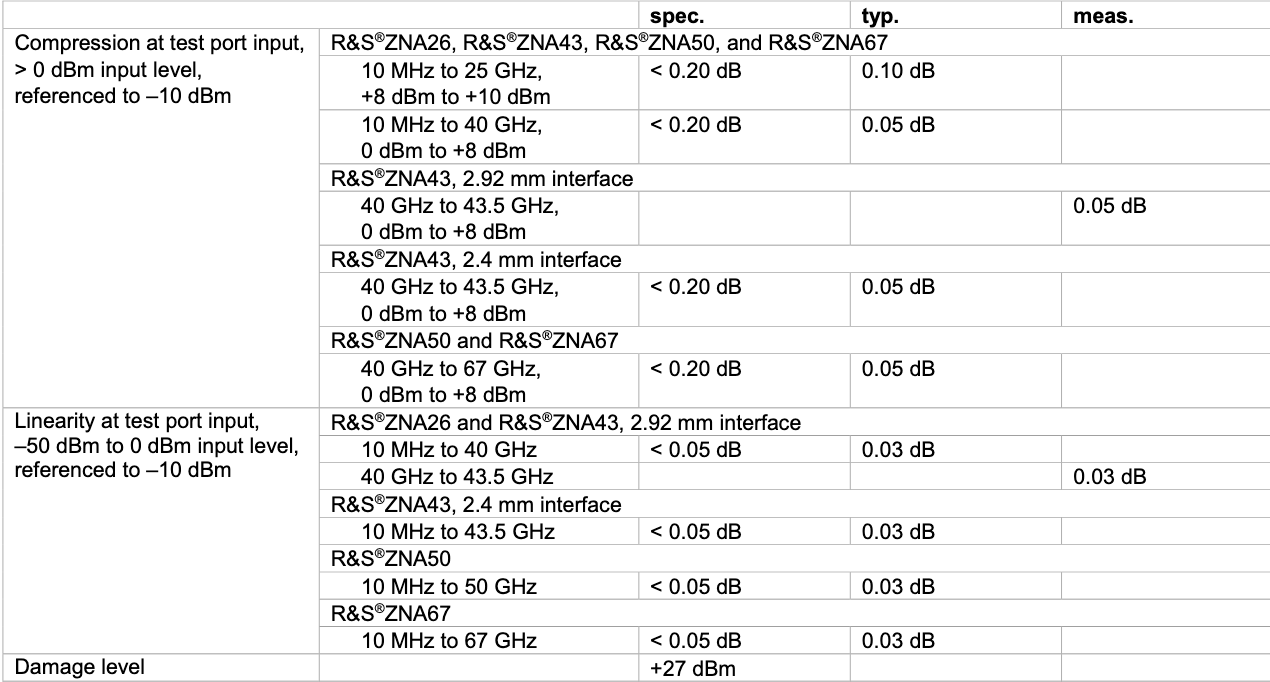
\includegraphics[keepaspectratio]{ZNA67_max_damage_level.png}}

}

\caption{title}

\end{figure}%

\subsubsection{c) Determine the maximum allowed output power of a
network analyzer for the amplifier of Task 8 without damaging the
VNA.}\label{c-determine-the-maximum-allowed-output-power-of-a-network-analyzer-for-the-amplifier-of-task-8-without-damaging-the-vna.}

Used
\href{https://www.alldatasheet.com/datasheet-pdf/download/103781/RFMD/NLB-300.html}{Datasheet
of NLB-300}

The maximum allowed output power of the analyzer is limited to the
maximum input values from the LNA. Here the datasheet states that
\(+20dBm\). But it has to be considered that the LNA is at its maximum
designed specifications. At this input level we exceed parameters like
1dB-Compression point depending on the frequency at \(\approx 13dBm\).

\subsection{Task 3}\label{task-3}

\subsubsection{How do the 16-term, 12-term and 8-term error models
differ? Specify the conditions that are assumed to apply to
each.}\label{how-do-the-16-term-12-term-and-8-term-error-models-differ-specify-the-conditions-that-are-assumed-to-apply-to-each.}

When measuring S-parameters using a VNA, imperfections in the
instrument, cables, and switching system introduce systematic errors. To
correct for these, mathematical error models are used during
calibration. Depending on the level of precision required and the type
of measurement setup, different models are applied. The errors are:

\begin{longtable}[]{@{}
  >{\raggedright\arraybackslash}p{(\linewidth - 8\tabcolsep) * \real{0.2400}}
  >{\raggedright\arraybackslash}p{(\linewidth - 8\tabcolsep) * \real{0.5000}}
  >{\centering\arraybackslash}p{(\linewidth - 8\tabcolsep) * \real{0.0900}}
  >{\centering\arraybackslash}p{(\linewidth - 8\tabcolsep) * \real{0.0900}}
  >{\centering\arraybackslash}p{(\linewidth - 8\tabcolsep) * \real{0.0800}}@{}}
\toprule\noalign{}
\begin{minipage}[b]{\linewidth}\raggedright
Error Term
\end{minipage} & \begin{minipage}[b]{\linewidth}\raggedright
Meaning / Description
\end{minipage} & \begin{minipage}[b]{\linewidth}\centering
16-Term
\end{minipage} & \begin{minipage}[b]{\linewidth}\centering
12-Term
\end{minipage} & \begin{minipage}[b]{\linewidth}\centering
8-Term
\end{minipage} \\
\midrule\noalign{}
\endhead
\bottomrule\noalign{}
\endlastfoot
e00 / e33 & Directivity (Fwd / Rev) & ✅ & ✅ & ✅ \\
e11 / e22 & Source Match (Fwd / Rev) & ✅ & ✅ & ✅ \\
e10·e01 / e23·e32 & Reflection Tracking (Fwd / Rev) & ✅ & ✅ & ✅ \\
e22 / e11 & Load Match (Fwd / Rev) & ✅ & ✅ & \\
e10·e32 / e23·e01 & Transmission Tracking (Fwd / Rev) & ✅ & ✅ & ✅ \\
& Crosstalk / Isolation (Fwd / Rev) & ✅ & & \\
\end{longtable}

\begin{itemize}
\tightlist
\item
  \textbf{Directivity} (Forward/Reverse): Measures how well the VNA can
  separate incident from reflected waves. E.g. isolate forward-going
  signals from the reverse signals induced by mismatches
\item
  \textbf{Source Match}: Represents mismatch between the VNA's source
  port and the DUT. Affects how much of the signal reflects back.
\item
  \textbf{Reflection Tracking}: Accounts for frequency response and
  losses in the signal path when measuring reflections.
\item
  \textbf{Load Match}: Represents mismatch at the DUT output or
  receiving port. Affects transmission accuracy.
\item
  \textbf{Transmission Tracking}: Similar to Reflection Tracking, but
  with also with the error from DUT to VNA
\end{itemize}

Here we can see the Terms in a 12-Term meassurement {[}5{]}:
\pandocbounded{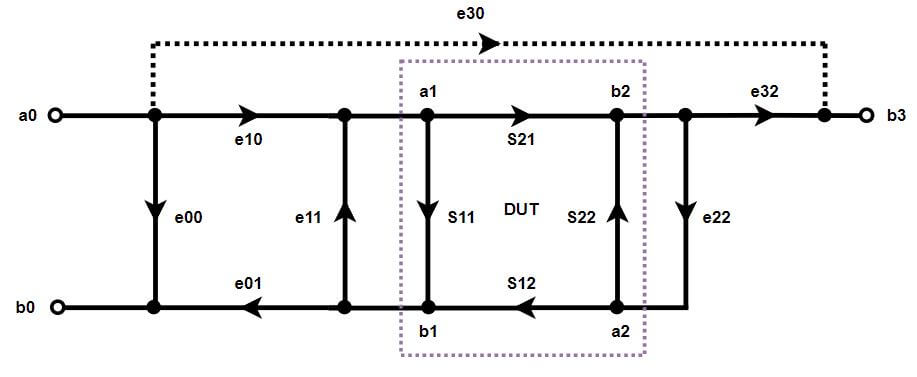
\includegraphics[keepaspectratio]{12TermForward.jpg}}
\pandocbounded{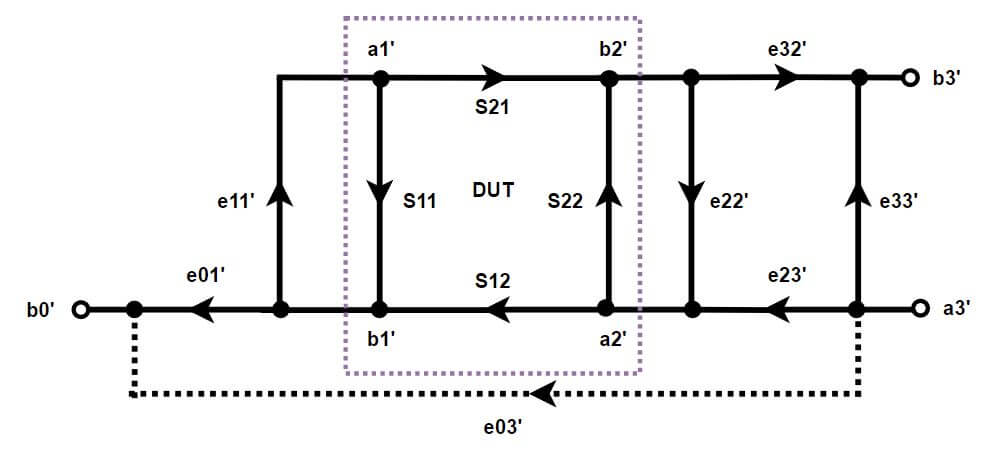
\includegraphics[keepaspectratio]{12TermReverse.jpg}}

And here the three methods are compared to each other:

\begin{longtable}[]{@{}
  >{\raggedright\arraybackslash}p{(\linewidth - 8\tabcolsep) * \real{0.2400}}
  >{\raggedright\arraybackslash}p{(\linewidth - 8\tabcolsep) * \real{0.5000}}
  >{\centering\arraybackslash}p{(\linewidth - 8\tabcolsep) * \real{0.0900}}
  >{\centering\arraybackslash}p{(\linewidth - 8\tabcolsep) * \real{0.0900}}
  >{\centering\arraybackslash}p{(\linewidth - 8\tabcolsep) * \real{0.0800}}@{}}
\toprule\noalign{}
\begin{minipage}[b]{\linewidth}\raggedright
Assumptions
\end{minipage} & \begin{minipage}[b]{\linewidth}\raggedright
Meaning / Description
\end{minipage} & \begin{minipage}[b]{\linewidth}\centering
16-Term
\end{minipage} & \begin{minipage}[b]{\linewidth}\centering
12-Term
\end{minipage} & \begin{minipage}[b]{\linewidth}\centering
8-Term
\end{minipage} \\
\midrule\noalign{}
\endhead
\bottomrule\noalign{}
\endlastfoot
Assumes Symmetry & Hardware is reciprocal & & ✅ & ✅ \\
Assumes Isolation & No Crosstalk & & & ✅ \\
Assumes Identical Ports & Ports behave identically & & & ✅ \\
\end{longtable}

\subsection{Task 4}\label{task-4}

\subsubsection{Why is a cable usually standardized to 50 Ohm in
microwave technology? What are the
advantages?}\label{why-is-a-cable-usually-standardized-to-50-ohm-in-microwave-technology-what-are-the-advantages}

\textbf{50\,Ω} is a standardized impedance because it represents a
compromise between two competing performance metrics:

\begin{itemize}
\tightlist
\item
  \textbf{Maximum power handling} (optimized near \textbf{30\,Ω})\\
\item
  \textbf{Minimum conductor loss} (optimized near \textbf{77\,Ω})
\end{itemize}

\begin{center}\rule{0.5\linewidth}{0.5pt}\end{center}

\paragraph{Maximum Power Handling}\label{maximum-power-handling}

The peak power is limited by the \textbf{electric field strength} at the
inner conductor, which must not exceed the dielectric breakdown limit.

Electric field at the inner conductor:

\[
E_{\text{max}} = \frac{V}{a \ln(b/a)}
\]

Solving for the maximum voltage before breakdown \$ E\_\{\text{break}\}
\$:

\[
V_{\text{max}} = E_{\text{break}} \cdot a \ln(b/a)
\]

Power delivered to a matched load:

\[
P = \frac{V_{\text{max}}^2}{2Z_0}
\]

Substitute for ( V\_\{\text{max}\} ):

\[
P \propto \frac{a^2 \ln^2(b/a)}{Z_0}
\]

From the impedance formula:

\[
Z_0 = \frac{60}{\sqrt{\varepsilon_r}} \ln(b/a)
\Rightarrow
P \propto \frac{a^2 \ln(b/a)}{60}
\]

This expression peaks near \$ Z\_0 \approx 30~\Omega \$, where the cable
supports \textbf{maximum power} before dielectric breakdown.

\begin{center}\rule{0.5\linewidth}{0.5pt}\end{center}

\paragraph{Minimum Attenuation}\label{minimum-attenuation}

In the low-loss approximation, the attenuation constant is:

\[
\alpha \approx \frac{R_s}{2Z_0} \left( \frac{1}{a} + \frac{1}{b} \right)
\]

Using:

\[
Z_0 = \frac{60}{\sqrt{\varepsilon_r}} \ln(b/a)
\]

We substitute and minimize \$ \alpha \$ with respect to the ratio \$
\frac{b}{a} \$. The optimal value for \textbf{minimum attenuation} is:

\[
Z_0 \approx 77\ \Omega
\]

\begin{center}\rule{0.5\linewidth}{0.5pt}\end{center}

The choice of \textbf{50\,Ω} impedance is a practical engineering
compromise:

\begin{itemize}
\tightlist
\item
  Closer to \textbf{30\,Ω} for good power handling\\
\item
  Close enough to \textbf{77\,Ω} for relatively low conductor loss. Some
  applications like TV infrastructure, where \(75\Omega\) is often used
  to prioritize this.
\end{itemize}

This makes 50\,Ω a well-balanced standard for \textbf{RF/microwave}
applications.

Here we visualize the conductor losses and power handling across the
Impedance:

\begin{Shaded}
\begin{Highlighting}[]
\NormalTok{b }\OperatorTok{=} \FloatTok{1.0}  \CommentTok{\# outer conductor radius (normalized)}
\NormalTok{epsilon\_r }\OperatorTok{=} \FloatTok{1.0}  \CommentTok{\# air dielectric constant}
\end{Highlighting}
\end{Shaded}

\begin{Shaded}
\begin{Highlighting}[]
\NormalTok{a }\OperatorTok{=}\NormalTok{ np.linspace(}\FloatTok{0.01}\NormalTok{, }\FloatTok{0.9} \OperatorTok{*}\NormalTok{ b, }\DecValTok{500}\NormalTok{)}
\NormalTok{ln\_ba }\OperatorTok{=}\NormalTok{ np.log(b }\OperatorTok{/}\NormalTok{ a)}

\NormalTok{Z0 }\OperatorTok{=} \DecValTok{60} \OperatorTok{/}\NormalTok{ np.sqrt(epsilon\_r) }\OperatorTok{*}\NormalTok{ ln\_ba}
\NormalTok{Vmax }\OperatorTok{=}\NormalTok{ a }\OperatorTok{*}\NormalTok{ ln\_ba}
\NormalTok{P }\OperatorTok{=}\NormalTok{ Vmax}\OperatorTok{**}\DecValTok{2} \OperatorTok{/}\NormalTok{ (}\DecValTok{2} \OperatorTok{*}\NormalTok{ Z0)}
\NormalTok{P\_normalized }\OperatorTok{=}\NormalTok{ P }\OperatorTok{/}\NormalTok{ np.}\BuiltInTok{max}\NormalTok{(P)}

\NormalTok{alpha }\OperatorTok{=}\NormalTok{ (}\DecValTok{1} \OperatorTok{/}\NormalTok{ Z0) }\OperatorTok{*}\NormalTok{ (}\DecValTok{1} \OperatorTok{/}\NormalTok{ a }\OperatorTok{+} \DecValTok{1} \OperatorTok{/}\NormalTok{ b)}
\NormalTok{alpha\_normalized }\OperatorTok{=}\NormalTok{ alpha }\OperatorTok{/}\NormalTok{ np.}\BuiltInTok{min}\NormalTok{(alpha)}
\end{Highlighting}
\end{Shaded}

\begin{Shaded}
\begin{Highlighting}[]
\NormalTok{plt.figure(figsize}\OperatorTok{=}\NormalTok{(}\DecValTok{9}\NormalTok{, }\DecValTok{6}\NormalTok{))}
\NormalTok{plt.plot(Z0, P\_normalized, label}\OperatorTok{=}\StringTok{\textquotesingle{}Normalized Max Power\textquotesingle{}}\NormalTok{, color}\OperatorTok{=}\StringTok{\textquotesingle{}blue\textquotesingle{}}\NormalTok{)}
\NormalTok{plt.plot(Z0, alpha\_normalized, label}\OperatorTok{=}\StringTok{\textquotesingle{}Normalized Attenuation\textquotesingle{}}\NormalTok{, color}\OperatorTok{=}\StringTok{\textquotesingle{}orange\textquotesingle{}}\NormalTok{)}

\NormalTok{plt.axvline(}\DecValTok{30}\NormalTok{, color}\OperatorTok{=}\StringTok{\textquotesingle{}blue\textquotesingle{}}\NormalTok{, linestyle}\OperatorTok{=}\StringTok{\textquotesingle{}{-}{-}\textquotesingle{}}\NormalTok{, label}\OperatorTok{=}\StringTok{\textquotesingle{}Max Power ≈ 30 Ω\textquotesingle{}}\NormalTok{)}
\NormalTok{plt.axvline(}\DecValTok{77}\NormalTok{, color}\OperatorTok{=}\StringTok{\textquotesingle{}orange\textquotesingle{}}\NormalTok{, linestyle}\OperatorTok{=}\StringTok{\textquotesingle{}{-}{-}\textquotesingle{}}\NormalTok{, label}\OperatorTok{=}\StringTok{\textquotesingle{}Min Attenuation ≈ 77 Ω\textquotesingle{}}\NormalTok{)}
\NormalTok{plt.axvline(}\DecValTok{50}\NormalTok{, color}\OperatorTok{=}\StringTok{\textquotesingle{}green\textquotesingle{}}\NormalTok{, linestyle}\OperatorTok{=}\StringTok{\textquotesingle{}{-}{-}\textquotesingle{}}\NormalTok{, label}\OperatorTok{=}\StringTok{\textquotesingle{}Standard = 50 Ω\textquotesingle{}}\NormalTok{)}

\NormalTok{plt.xlabel(}\StringTok{\textquotesingle{}Characteristic Impedance (Ω)\textquotesingle{}}\NormalTok{)}
\NormalTok{plt.ylabel(}\StringTok{\textquotesingle{}Normalized Value\textquotesingle{}}\NormalTok{)}
\NormalTok{plt.title(}\StringTok{\textquotesingle{}Power Handling and Attenuation vs Characteristic Impedance\textquotesingle{}}\NormalTok{)}
\NormalTok{plt.grid(}\VariableTok{True}\NormalTok{)}
\NormalTok{plt.legend()}
\NormalTok{plt.tight\_layout()}
\NormalTok{plt.show()}
\end{Highlighting}
\end{Shaded}

\pandocbounded{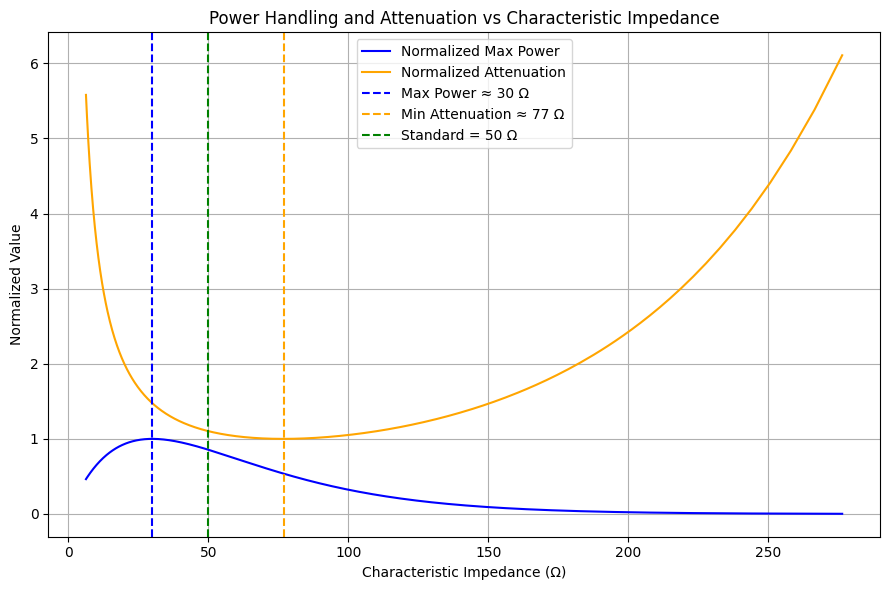
\includegraphics[keepaspectratio]{Lab1_Preliminary_files/figure-pdf/cell-5-output-1.png}}

{[}1{]}
https://www.microwaves101.com/encyclopedias/coax-loss-calculations
{[}2{]} https://www.microwaves101.com/encyclopedias/why-fifty-ohms
{[}3{]}
https://www.allaboutcircuits.com/technical-articles/introduction-to-vna-calibration-techniques/
{[}4{]}
https://www.allaboutcircuits.com/technical-articles/understanding-the-12-term-error-model-and-solt-calibration-method-for-vna-measurements/
{[}5{]} http://emlab.uiuc.edu/ece451/appnotes/Rytting\_NAModels.pdf
{[}6{]}
https://coppermountaintech.com/introduction-to-the-metrology-of-vna-measurement/
{[}7{]} Doug Rytting, ``Network Analyzer Error Models and Calibration
Methods,'' Agilent Technologies, White Paper, 1998. Available in:
http://emlab.uiuc.edu/ece451/appnotes/Rytting\_NAModels.pdf {[}8{]} Z.
Peterson, ``The Mysterious 50 Ohm Impedance: Where It Came From and Why
We Use It,'' Altium Resources, March 4, 2021. {[}Online{]}. Available:
https://resources.altium.com/p/mysterious-50-ohm-impedance-where-it-came-and-why-we-use-it




\end{document}
